\chapter{Dataset and Methodology}
\label{ch:method}

\section{The AG News corpus}

AG News is a topic classification benchmark derived from the AG corpus of news articles, introduced
in its current form by Zhang et al.\ \cite{zhang2015}. Each record consists of a class index, a
headline and a short description. The four classes are balanced by construction.

\begin{table}[ht]
\centering
\caption{Composition of the AG News corpus as distributed.}
\label{tab:corpus}
\begin{tabular}{lrr}
\toprule
\textbf{Split} & \textbf{Records} & \textbf{Per class} \\
\midrule
Training file & 120{,}000 & 30{,}000 \\
Test file     & 7{,}600   & 1{,}900 \\
\midrule
Total         & 127{,}600 & 31{,}900 \\
\bottomrule
\end{tabular}
\end{table}

The corpus was obtained programmatically through the Kaggle API from the dataset
\code{amananandrai/ag-news-classification-dataset}, so that acquisition is reproducible rather than
dependent on a manual download. The four class indices map to \emph{World}, \emph{Sports},
\emph{Business} and \emph{Science/Technology} respectively.

The text field used throughout is the concatenation of headline and description:
\begin{equation*}
\text{text} = \text{Title} \;+\; \text{``.\,''} \;+\; \text{Description}.
\end{equation*}

\section{Data cleaning}
\label{sec:cleaning}

Inspection of the raw CSV files revealed a systematic artefact inherited from the original scrape.
Escape sequences appear \emph{literally} in the text rather than as the control characters they
denote. A representative record reads:

\begin{quote}
\code{Reuters - Short-sellers, Wall Street's dwindling\bs band of ultra-cynics, are
seeing green again.}
\end{quote}

Here \code{\bs b} is a literal backslash followed by the letter \code{b}, not a
backspace. The phrase should read \emph{``dwindling band of ultra-cynics''}.

This is not a cosmetic problem. Under the tokenisation scheme described in
Section~\ref{sec:tokenisation}, the backslash is discarded as a non-matching character and the
surrounding letters are welded into the single token \code{dwindlingband}. Two genuine, frequent
words are replaced by one spurious type that occurs almost nowhere else in the corpus and is
therefore pruned by the minimum-frequency cutoff, mapping to the unknown token at both training and
test time. The net effect is the silent destruction of lexical evidence in exactly the kind of
content-bearing position that matters most for topic classification.

The cleaning step applies the regular expression \code{\bs\bs[a-z]},
replacing each such sequence with a single space, followed by whitespace normalisation. This is
applied identically to both the training and test files, before any split is taken.

\keypoint{Methodological note.} This artefact is easy to overlook, because a model trained on the
uncleaned data still trains and still reports a plausible accuracy. The discovery came from reading
the raw records directly rather than from any error signal. It is reported here because it is
representative of a general principle in applied machine learning: a substantial fraction of
achievable performance is determined before any model is defined.

\section{Experimental design}

\subsection{The controlled subset}

The case-study brief specifies the use of approximately 60{,}000 records for a controlled
experiment. This was implemented as a stratified sample of exactly 15{,}000 records per class drawn
from the 120{,}000-record training file with a fixed random seed, subsequently shuffled and split
into training and validation partitions.

\begin{table}[ht]
\centering
\caption{Data splits used in the experiment. The test set is the full official file and is used
once, for the final evaluation reported in Chapter~\ref{ch:results}.}
\label{tab:splits}
\begin{tabular}{lrrl}
\toprule
\textbf{Split} & \textbf{Records} & \textbf{Per class} & \textbf{Purpose} \\
\midrule
Training   & 54{,}000 & 13{,}500 & parameter estimation \\
Validation & 6{,}000  & 1{,}500  & early stopping, learning-rate selection \\
Test       & 7{,}600  & 1{,}900  & final evaluation only \\
\bottomrule
\end{tabular}
\end{table}

All three partitions are exactly class-balanced, so accuracy and macro-averaged $F_1$
are directly interpretable and a majority-class baseline sits at 25\%.

\subsection{The four experimental controls}

The comparison is designed so that architecture is the only free variable. Four quantities are held
fixed.

\begin{enumerate}
\item \textbf{Data.} One subset, one split, one fixed seed. Both models see identical records in an
      identical order.

\item \textbf{Preprocessing.} One tokeniser, one vocabulary, one maximum sequence length. The
      integer tensors fed to the two models are not merely equivalent --- they are the same
      objects.

\item \textbf{Capacity.} Both models are sized to approximately 265{,}000 non-embedding
      parameters, a difference of 0.19\%. Without this control, any observed difference could be
      attributed to model size rather than architecture.

\item \textbf{Training budget.} Identical batch size, epoch cap, optimiser family, weight decay,
      gradient clipping, early-stopping criterion and random seed.
\end{enumerate}

\subsection{The one quantity that is not shared}

The learning rate differs between the two models: $10^{-3}$ for the recurrent model and
$3\times10^{-4}$ for the Transformer. Both values were selected on the validation split and never
on the test set.

This choice warrants explicit defence, since it appears to weaken the control. Imposing a single
shared learning rate would \emph{appear} fairer, but it would in fact handicap whichever
architecture that particular value suited less well, and the experiment would then measure
sensitivity to one arbitrary hyperparameter rather than the architectures themselves. Recurrent
and self-attentive models are known to have different stable learning-rate regimes. The quantity
that is properly controlled is the \emph{compute budget}; the learning rate is a per-architecture
tuning decision made on data that is not used for evaluation.

\section{Preprocessing}
\label{sec:tokenisation}

\subsection{Tokenisation}

Documents are lowercased and tokenised with the regular expression
\code{[a-z0-9']+}, which extracts maximal runs of alphanumeric characters and apostrophes. This
retains contractions and possessives as single tokens while discarding punctuation.

The tokeniser is deliberately simple. A more sophisticated scheme --- subword segmentation, for
instance --- would very likely improve both models. It is omitted precisely because both models
must receive identical input: any tokeniser sophistication is a confound if it happens to suit one
architecture better than the other. The simple scheme makes the comparison clean at a small cost in
absolute accuracy.

\subsection{Vocabulary}

The vocabulary is constructed from the \emph{training split only}. Neither the validation nor the
test text contributes any token to the vocabulary, which eliminates a subtle and common form of
information leakage.

Types occurring fewer than twice in the training split are discarded. Two special tokens are
reserved: index $0$ for padding and index $1$ for unknown tokens. The resulting vocabulary contains
\textbf{33{,}964} types.

\subsection{Sequence length}

Choosing a maximum sequence length is a trade-off between truncating information and wasting
computation on padding. The choice was made from the measured distribution rather than by
convention.

\begin{table}[ht]
\centering
\caption{Token-length statistics of the training split.}
\label{tab:lengths}
\begin{tabular}{lr}
\toprule
\textbf{Statistic} & \textbf{Tokens} \\
\midrule
Median                  & 39 \\
Mean                    & 39.4 \\
95th percentile         & 58 \\
Maximum                 & 181 \\
\midrule
Chosen \code{MAX\us{}LEN}  & 64 \\
Coverage at this length & 96.94\% \\
\bottomrule
\end{tabular}
\end{table}

Figure~\ref{fig:lengths} shows the full distribution. A cutoff of 64 tokens leaves 96.94\% of
training documents untruncated while keeping the sequence dimension small enough for the recurrent
model to remain tractable on CPU.

\begin{figure}[ht]
\centering
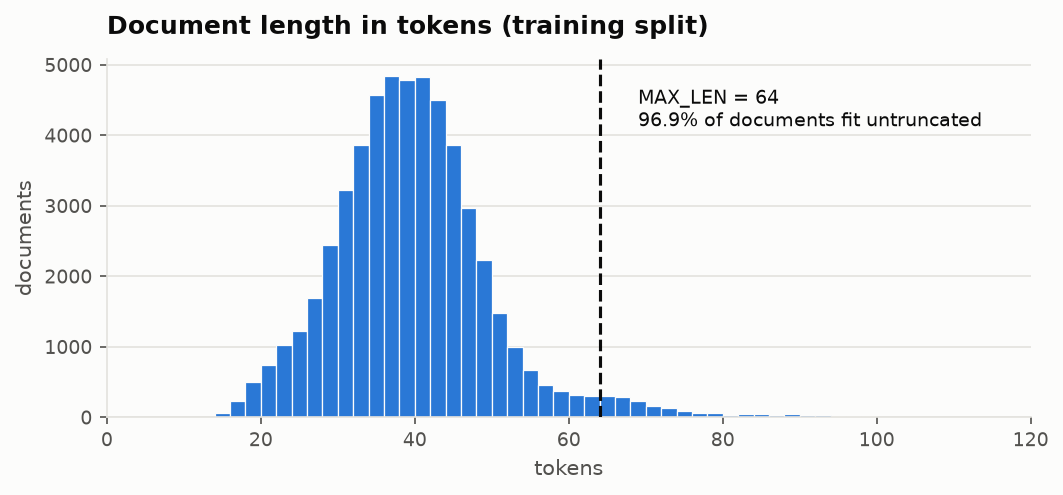
\includegraphics[width=0.92\textwidth]{figures/fig0_token_lengths.png}
\caption[Distribution of document lengths]{Distribution of document lengths in tokens on the
training split. The dashed line marks the chosen cutoff of 64 tokens. The distribution is tightly
concentrated around a median of 39 tokens --- the property that, as argued in
Chapter~\ref{ch:discussion}, accounts for the equivalence of the two architectures.}
\label{fig:lengths}
\end{figure}

\keypoint{The central statistic of this study.} The median document is 39 tokens long. Every
substantive conclusion in Chapter~\ref{ch:discussion} follows from this number.

\subsection{Encoding}

Each document is converted to a fixed-length vector of 64 integer indices, truncated or
right-padded with the padding index as required, together with its true length. Documents reducing
to zero tokens are mapped to a single unknown token so that no sequence has a zero-length mask.

\section{Evaluation metrics}

\subsection{Accuracy and $F_1$}

Since all splits are exactly balanced, accuracy is a meaningful primary metric. It is nonetheless
reported alongside per-class precision, recall and $F_1$:
\begin{equation}
P_c = \frac{TP_c}{TP_c + FP_c}, \qquad
R_c = \frac{TP_c}{TP_c + FN_c}, \qquad
F1_c = \frac{2 P_c R_c}{P_c + R_c}.
\end{equation}

Macro-averaged $F_1$ --- the unweighted mean of the per-class values --- is used as
the model selection criterion, because it weights all four classes equally and is sensitive to
failure on any single class in a way that accuracy is not.

\subsection{Confusion matrix}

The $4\times4$ confusion matrix is reported row-normalised, so that entry $(i,j)$ gives the
proportion of true class $i$ predicted as class $j$. With four classes there are twelve
off-diagonal cells, and their structure is considerably more informative about model behaviour
than any scalar summary.

\subsection{McNemar's test}
\label{sec:mcnemar}

Comparing two classifiers on the same test set produces \emph{paired} observations, and a test
that respects the pairing is required. McNemar's test \cite{mcnemar1947} considers only the
discordant cases --- documents on which the two models disagree --- arranged as:

\begin{table}[ht]
\centering
\caption{Contingency structure for McNemar's test.}
\label{tab:mcnemar_structure}
\begin{tabular}{lcc}
\toprule
 & \textbf{Model B correct} & \textbf{Model B wrong} \\
\midrule
\textbf{Model A correct} & $a$ & $b$ \\
\textbf{Model A wrong}   & $c$ & $d$ \\
\bottomrule
\end{tabular}
\end{table}

The counts $a$ and $d$ --- cases where both models agree --- carry no information about which model
is better and are discarded. Under the null hypothesis that the two models have equal error rates,
each discordant case is equally likely to fall in cell $b$ or cell $c$, so
\begin{equation}
b \sim \operatorname{Binomial}(b + c,\; 0.5).
\end{equation}
The exact binomial test on this statistic is used here in preference to the chi-squared
approximation, since it is valid for any count.

\keypoint{Why this matters.} Accuracy differences below one percentage point are routinely reported
as improvements in the literature. On a 7{,}600-document test set, a difference of 0.09 percentage
points corresponds to seven documents. Without a paired significance test there is no principled
basis for distinguishing such a difference from sampling noise, and as Chapter~\ref{ch:results}
shows, in this case it cannot be so distinguished.

\section{Experimental environment}

\begin{table}[ht]
\centering
\caption{Hardware and software environment. All timing results in Chapter~\ref{ch:results} are
specific to this configuration.}
\label{tab:environment}
\begin{tabular}{ll}
\toprule
\textbf{Component} & \textbf{Specification} \\
\midrule
Processor        & 12 logical cores, 6 PyTorch threads \\
Accelerator      & none --- CPU execution only \\
Memory           & 15\,GB \\
Operating system & Linux (Fedora, kernel 6.17) \\
Python           & 3.14.8 \\
PyTorch          & 2.15.0 (CPU build) \cite{paszke2019} \\
Random seed      & 42, applied to \code{random}, \code{numpy} and \code{torch} \\
\bottomrule
\end{tabular}
\end{table}

The absence of a GPU is not incidental to the findings. It materially affects the cost comparison
in Section~\ref{sec:cost}, and the discussion there is explicit about which conclusions are
hardware-dependent.
